\documentclass[conference]{IEEEtran}
\IEEEoverridecommandlockouts
% The preceding line is only needed to identify funding in the first footnote. If that is unneeded, please comment it out.
\usepackage{cite}
\usepackage{amsmath,amssymb,amsfonts}
\usepackage{algorithmic}
\usepackage{graphicx}
\usepackage{textcomp}
\usepackage{xcolor}
\def\BibTeX{{\rm B\kern-.05em{\sc i\kern-.025em b}\kern-.08em
    T\kern-.1667em\lower.7ex\hbox{E}\kern-.125emX}}
\begin{document}

\newcommand{\linebreakand}{%
  \end{@IEEEauthorhalign}
  \hfill\mbox{}\par
  \mbox{}\hfill\begin{@IEEEauthorhalign}
}

\title{Autonomous Systems Group Pi\\
}

\author{\IEEEauthorblockN{1\textsuperscript{st} Benedikt Fischhaber}
\IEEEauthorblockA{\textit{Technical University of Munich} \\
Munich, Germany \\
benedikt.fischhaber@tum.de}
\and
\IEEEauthorblockN{2\textsuperscript{nd} Maximilian Miller}
\IEEEauthorblockA{\textit{Technical University of Munich} \\
Munich, Germany \\
maxi.miller@tum.de}
\and
\IEEEauthorblockN{3\textsuperscript{rd} Samuel Zeitler}
\IEEEauthorblockA{\textit{Technical University of Munich} \\
Munich, Germany \\
samuel.zeitler@tum.de}
\linebreakand
\IEEEauthorblockN{4\textsuperscript{th} Divij Grover}
\IEEEauthorblockA{\textit{Technical University of Munich} \\
Munich, Germany \\
ge56jic@mytum.de}
\and
\IEEEauthorblockN{5\textsuperscript{th} Nicholas Poggendorf}
\IEEEauthorblockA{\textit{Technical University of Munich} \\
Munich, Germany \\
nicholas.poggendorf@tum.de}
}


\maketitle

\begin{abstract}
This document is the documentation of the autonomous systems project of Team Pi. It describes the goal of the project, the functional components of the code, their implementation and the interaction of all components.
\end{abstract}

\section{Introduction}
For surviving an avalanche accident, time is key. Avalanche beacons are a widespread tool used by mountaineers for locating buried victims quickly. Each member of a hiking or skiing party wears a beacon module in transmitter setting close to his body. In case of an avalanche the rescuer turns his module to receiver mode. The rescuer than starts to move in a search pattern over the avalanche. If a signal is detected, a directional marker and a distance is indicated on the beacon sensor. The rescuer follows this indicator, which points in direction of the electromagnetic flux lines. In close proximity to the victim, only the distance is of relevance. The rescuer moves his receiver over the snow and approximates the position of the victim. Most sensors are capable of detecting a multitude of different transmitter signals.

Unmanned Aerial Vehicles (UAVs) equipped with beacon sensors have the potential to decrease the search time significantly. UAVs are commonly used by professional Search and Rescue (SAR) teams mostly for covering large and remote areas in search missions. The use of highly autonomous systems could release SAR personal from high physical loads, increase search efficiency and give access to otherwise unreachable areas. This work presents a way of simulating a UAV based search mission within the Robot Operating System (ROS) framework and the Unity game engine. 

\section{Mission description}
In the following a short description of the mission should be stated. A preset number of transmitters is randomly placed within a search area with predefined corners. Then the drone has to localize the beacons by hovering over their position in the defined search area. Initially, the drone follows a pre-planned search pattern, but as soon as a beacon is detected within sensor range, the drone executes a search strategy until the victim is found. It then returns to the original search pattern. When all victims have been found or the search area has been completely scanned, the drone returns to its starting point. Finally, a report should be provided on where the found victims are located.

\section{Information flow and software architecture}
As usual when using ROS, the code was structured into packages and nodes. In order to clarify the communication between the different nodes, the flow of information and communication will be briefly presented below. The exact implementation and function of the individual components is presented in the following chapters.
The entire communication and all messages exchanged between the nodes are shown in the following ros computation graph (rqt) graph in Fig. \ref{fig:rqt}.
\begin{figure}[htbp]
\centerline{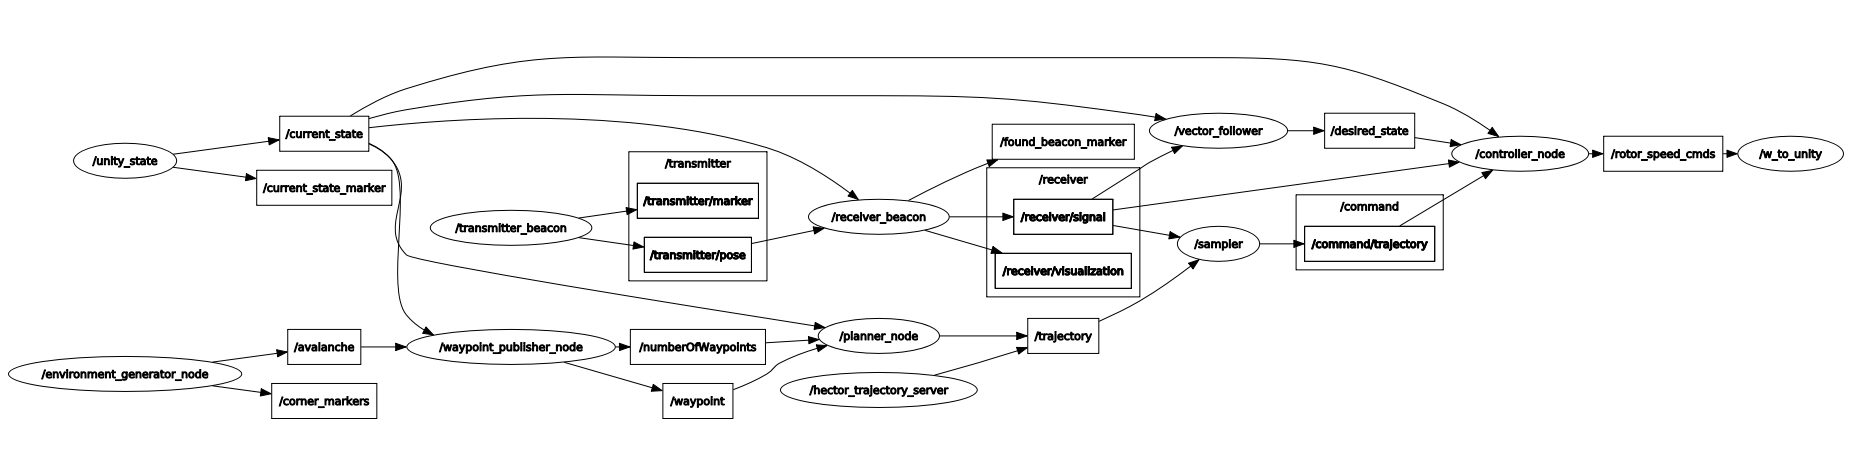
\includegraphics[width=1\columnwidth]{final_rqt_graph.png}}
\caption{ros computation graph}
\label{fig:rqt}
\end{figure}
To explain the rqt graph, the information flow is followed from left to right. We will mainly focus on those messages that contribute to the control flow of the drone. Messages for visualization are not explained in detail here. These contain in their name for example "visualization" or "marker".
The node unity\_state represents the connection to the given Unity simulation and sends the message current\_state, which contains the current state of the drone in the virtual environment. This message is received by several nodes.
At the beginning of the simulation, the transmitterNode reads the corners of the search area and the number of beacons from a yaml file. Then the positions of the beacons are randomly generated and sent to the receiverNode in the transmitter/pose message.
The receiverNode then uses these positions to simulate the magnetic field lines of the beacons at this location and thus the receiver of the drone. In doing so, the receiverNode permanently sends the receiver/signal message. This includes the distance to the next beacon that is within sensor range and a vector corresponding to the magnetic field of the beacon at the current position. If no sensor is in range, the distance -1 is sent.
The message /receiver/signal is received by the vector\_follower among others. This converts the received direction vector from the message of the receiver into a /desired\_state message.
In addition, at the beginning of the simulation, the environment\_generator\_node reads the positions of the corners of the search area from the yaml file. These positions are then sent as an /avalanche message to the waypoint\_publisher\_node.
In the waypoint\_publisher\_node a search pattern is then placed in the given search area. The generated waypoints and their number are then sent to the planner\_node as /waypoint and /numberOfWaypoints.
The planner\_node uses the given number of waypoints, the waypoints themselves and the current position of the drone to create a snap optimal trajectory. This is sent as a /trajectory message.
The sampler receives this trajectory and uses it to create the /command/trajectory message, which is received by the drone's controller and thus controls the drone's flight. The sampler also receives the /receiver/signal message from the receiver. If the distance contained therein is not equal to -1, then this is the signal to the sampler that a victim should now be sought. Thus no more commands are sent to the controller. Only when the victim has been found and the receiver sends the distance -1 again, commands are sent to the controller again.
The controller itself uses the messages /current\_state, /desired\_state, /receiver\_signal and /command/trajectory to calculate the velocities of the propellers and thus to control the drone. The same decision logic is used as in the sampler: If the distance in /receiver/signal is equal to -1, the commands of the sampler and therefore the predefined search pattern is followed. If the distance is not equal to -1, the /desired\_state message of the vector\_follower is used.
The last node in this whole chain is the w\_to\_unity node, which connects to the Unity environment and sends the commands to the virtual drone.
\section{Search pattern}
In order for the search pattern to be generated, we need to define the search area. The search area is a parallelogram with 4 corners. Those corners can be set within the src/environment\_generator/config/environment\_params.yaml file. They will then be read by the environment generator node which will create a ros-message containing the coordinates of the corners of the search area. Once the waypoint\_publisher\_node receives this message and made sure that the unity simulation is already running, the search pattern is generated. Using this approach the search area can easily be adjusted and the search pattern will always be calculated accordingly. The search pattern starts from the corner closest to the drone and covers the search area in an S-shape (see Fig. \ref{fig:searchPattern}). The distance between the horizontal lines is defined by the following equation: \begin{equation}
    dist = 2*sensorrange - overlap
\end{equation}
The sensor range corresponds to the distance upon which the beacons are detected by the sensor and the overlap is a parameter that can be adjusted. With the overlap parameter we can achieve multiple things: 1. A safety margin, that makes sure we don’t have unscanned stripes between turns. 2. A compensation for the additional distance to the beacons created by the height above ground. (see Fig. \ref{fig:heightComp}). The distance between the vertical lines is calculated by max(A-B, C-D). With the stepSize parameter the density of the waypoints can be adjusted. By decreasing this parameter, the amount of waypoints placed on the searching path increases. The S-curve is continued until all corners of the search area lie within the sensor range of a waypoint. The origin is added as the final waypoint of the pattern. The waypoints then are sent to the planner node where the snap trajectory is calculated.
\begin{figure}[htbp]
\centerline{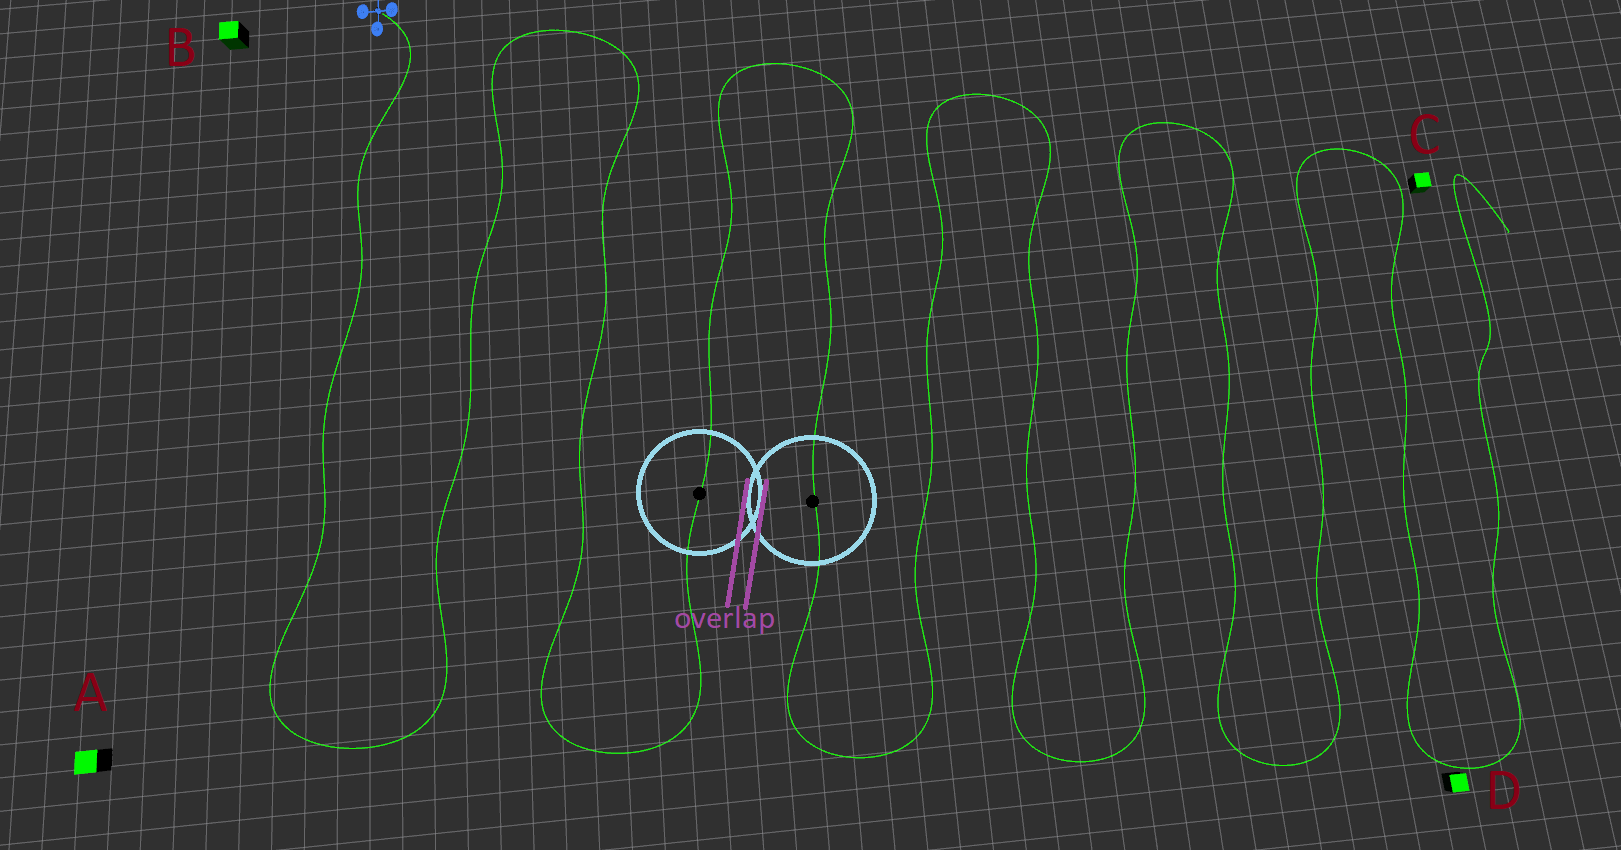
\includegraphics[width=1\columnwidth]{Searchpattern_withOverlap.png}}
\caption{Searchpattern}
\label{fig:searchPattern}
\end{figure}
\begin{figure}[htbp]
\centerline{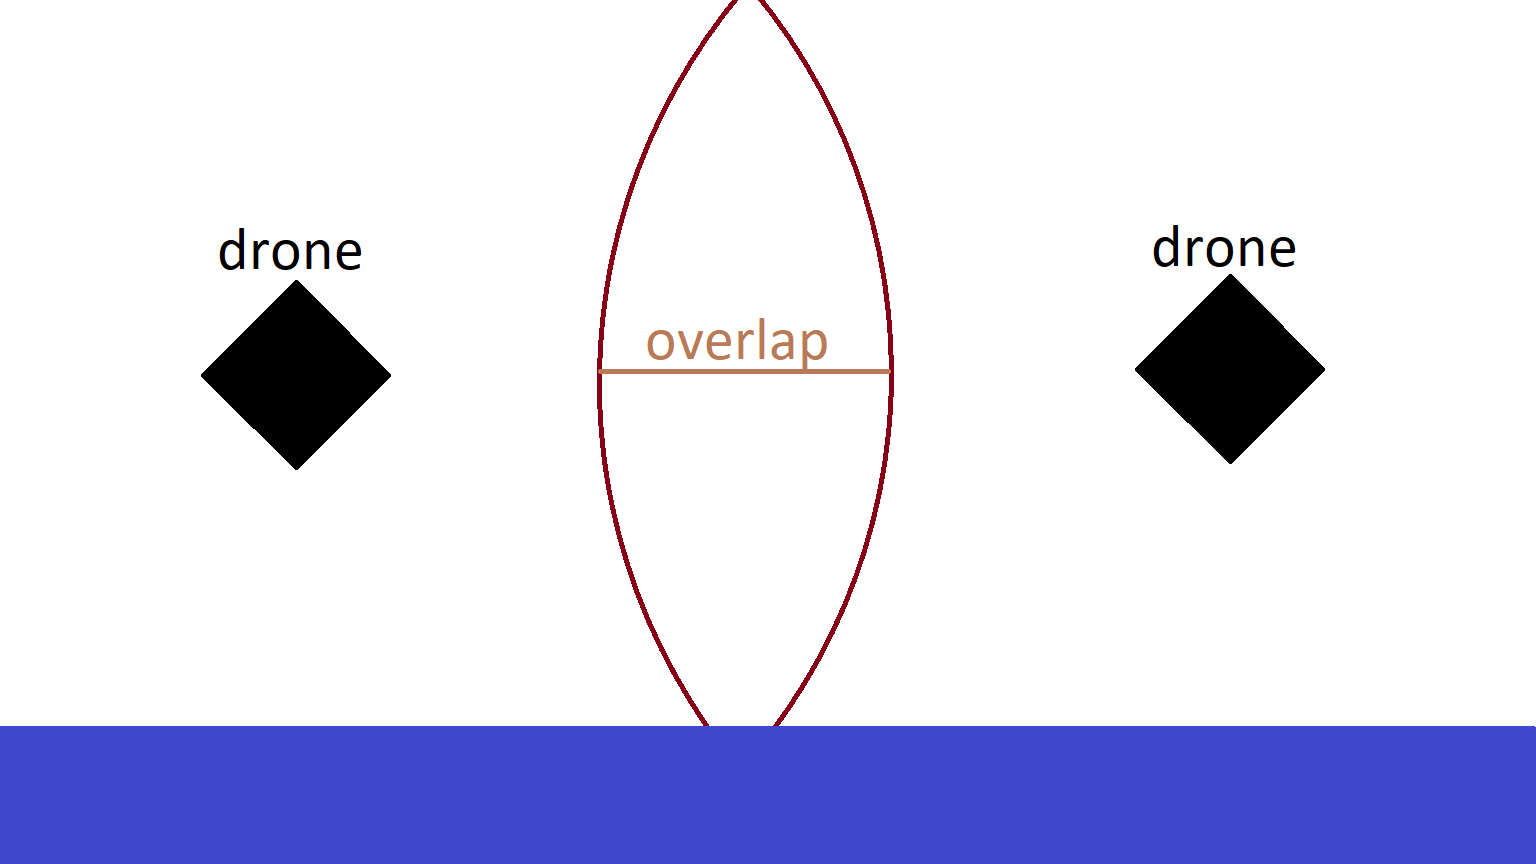
\includegraphics[width=1\columnwidth]{heightComp.png}}
\caption{Visualization of overlap and the influence of height above ground}
\label{fig:heightComp}
\end{figure}

\section{mission following}
After the mission has been planned, the drone must follow the calculated search pattern. For this purpose, functions from the package mav\_trajectory\_generation, which was written by the Autonomous Systems Lab at ETH Zurich\cite{b1}, are used in the planner. 
The waypoint\_publisher first sends the number of waypoints for the trajectory to the planner. Then, the planned waypoints for the search pattern are sent to the planner one by one. If the number of waypoints received matches the number of the message before, the trajectory is generated. For this purpose, the list of waypoints is passed to a nonlinear optimizer. This then calculates the snap optimal trajectory for the given points. Since the optimization is a very computationally intensive process, this can take some time. The exact duration depends on the computing power of the computer used.
Once a trajectory has been successfully generated, it is sent to the sampler, which is also part of the package mentioned above. The sampler then ensures that the trajectory received is sent to the drone's controller piece by piece. The sampler has been slightly modified to pause while searching for a victim within range.
The sampler also receives the /receiver/signal message from the receiver. If the distance contained in this message is greater than -1, the publish process in the sampler is stopped by pausing the timer that is responsible for publishing. If the received distance is -1 again, the timer is resumed.

\section{beacon simulation}
\label{beacon simulation}
An avalanche transceiver or avalanche beacon is a type of emergency locator beacon, which consists of a radio a transmitter and receiver. They are used as a one unit. There are two types of avalanche beacons: digital and analog. In this project, the digital transceivers are simulated. Digital transceivers (receiver) compute distance and direction to the buried transceiver (transmitter) with the help of strength of the signal and the dipole flux pattern. In this project beacons with three mutually perpendicular reception antennas are used. Because of the three perpendicular antennas they are able to measure the complete vector field. The antennas are attached to the drone, therefore the orientation of the antennas is considered same as of the drone. The reference frame of the receiver is denoted by \digamma{($O_r$ , $x_r$ , $y_r$ , $z_r$)}, and of the transmitter is indicated by \digamma{($O_t$ , $x_t$ , $y_t$ , $z_t$)}. The position of the transmitter and receiver is $p_t$ and $p_r$ respectively.  

There are three main steps to localize the victim, as shown in Fig. \ref{fig:beaconSearchPhases}.
\begin{itemize}
\item Phase 1 - Primary search:  This is the zone where the beacon signal is the weakest. Since, the distance between the receiver and transmitter is too long, the receiver is unable to recognize the Electromagnetic field and outputs no signal. The effect of the environment noise is too high to get any reliable information. Therefore, if the estimated distance is is greater than 5000 cm, the output vector flux and estimated distance is set to -1.
\begin{equation}
(\bar{q}_{flux}, d) = ([-1,-1,-1], -1)
\end{equation}

\begin{figure}[htbp]
\centerline{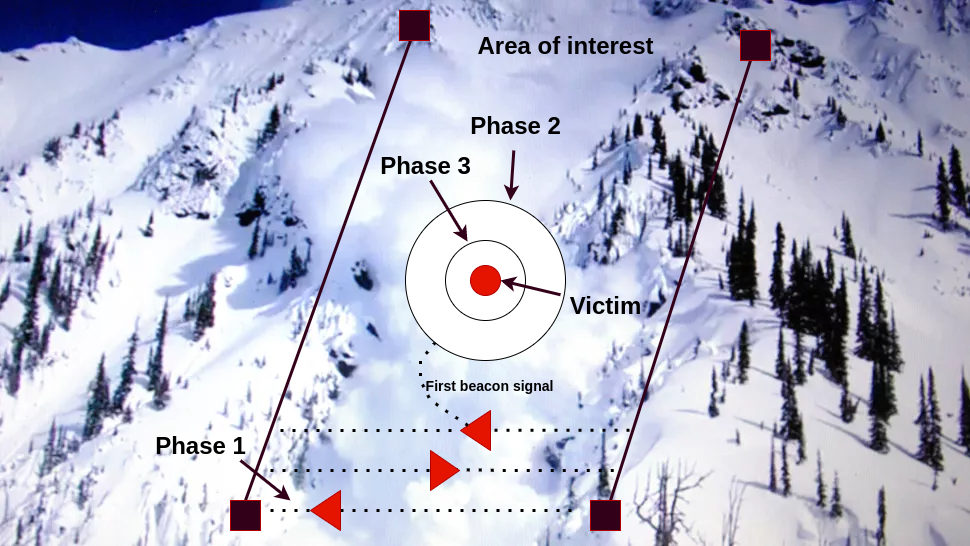
\includegraphics[width=1\columnwidth]{beacon_searchPattern.png}}
\caption{Beacon search phases}
\label{fig:beaconSearchPhases}
\end{figure}


\item Phase 2 - Coarse search: When approaching to the victim, one of the method is the directional search that
consists in following the direction of the magnetic field.
Since, all the flux lines must converge to the victim’s
antenna, the trajectory followed by the drone is curved as the flux line. The mathematical model of the magnetic vector field is given by \cite{b2}. The Electromagnetic flux lines are calculated using 3, 4 and 5. ${\bar{r}}$ is the position vector between transmitter and receiver, r is the euclidean distance between the receiver and transmitter,  $\bar{H}$ is the magnetic field strength,  $\bar{m}$ is the magnetic moment.

\begin{equation}
{\bar{r}} = \bar{p_t} - \bar{p_r}
\end{equation}

\begin{gather}
 A
 =
\begin{pmatrix}
   2r_x^2-r_y^2-r_z^2  & 3r_x r_y & 3r_x r_z \\
   3r_x r_y  & 2r_y^2-r_x^2-r_z^2  & 3r_y r_z \\
   3r_x r_z  & 3r_y r_z & 2r_z^2-r_x^2-r_y^2  \\
   \end{pmatrix}
\end{gather}

\begin{equation}
\ \bar{H} =  \frac{1}{4 \pi r^5} A { \bar{m}} 
\end{equation}
 
 
$\bar{H}$ is then normalised and transformed to the inertial frame and the resulting vector $\bar{H_b}$ points in the direction of magnetic flux and is sent as an output of the receiver node. The operating range of this zone d$\in$[500,5000] cm. The distance is calculated using the equation 6 \cite{b3}. {\kappa$_{eq}$} is constant tuned by the manufacturers and $L_{xy}$ represents the projector operator on the $x_r$, $y_r$ axes. The estimated distance d is determined by exploiting one of the most sensitive antennae.

\begin{equation}
d =  \left(\frac{\kappa_{eq} }{4 \pi \parallel L_{xy} \leftidx{^r} \bar{H_b}\parallel}\right) ^{\frac{1}{3}}
\end{equation}

Once the distance is less between in the range d$\in$[5000,500] cm, phase 2 is activated and starts sending the direction vector and the estimated distance of the beacon in range. The process continues until the locked beacon is either found or got lost during the search.

\item Phase 3 - Fine search:  In this zone the sensed electromagnetic flux lines is sufficiently strong and the all three antennae are utilized. The estimated distance is calculated using equation 7.   \cite{b3}

\begin{equation}
d =  \left(\frac{\kappa_{eq} }{4 \pi \parallel\leftidx{^r}\bar{H_b}\parallel}\right) ^{\frac{1}{3}}
\end{equation}
Once the drone reaches a threshold distance of 2.5 m, the receiver node assumes that the drone is found and an approximated location of transmitter is recorded. Since, the output depends on the orientation of the drone, sometimes the /receiver/signal node outputs unreliable data. In that case the last recorded reliable data is sent to the drone for at least 3 seconds. If drone is not able to locate the drone for the time period, the beacon is considered to be lost and the search continues. 

It has been found that the effect of environmental noise on the data is really high when the receiver is far away from the transceiver(d $\ge$ 50m). Since the data above 50 m is ignored, this helps to simulate the effects of the noise \cite{b3}.

\end{itemize}


\section{Trajectory execution}
At the beginning of the simulation, the drone will start following a search path after the initial planning is finished. As mentioned above, the search path consists of automatically generated waypoints from the waypoint\_publisher that aim to fully cover the specified avalanche area in a snake like manner. Once a beacon gets in the sensor range (50m), first a red arrow will start pointing in the direction of the detected flux. If the drone gets even closer to the beacon (35m), it will stop following its preplanned trajectory and will switch to vector-following. The margin of 15m between the first detection of the flux and the decision to start pursuing the beacon proofed as essential for a stable approach. 

Vector following:
During vector following, the drone is directly following the  direction of the detected flux. The speed is calculated as a function of the remaining distance to the beacon, to make sure that the drone is in a slow and steady approach when making its final measurement. Otherwise the the drone could miss the beacon or make an inaccurate estimation of the beacons position due to fluctuations in the field lines. The location of the beacon is then reported by the drone together with the estimated localisation error represented as a sphere in rviz.

The speed is calculated with the following formula: 

\begin{equation}
\parallel{\bar{v}_{drone}}\parallel = {max(0.5,min(2, \frac{distance}{500}))}
\end{equation}

\begin{figure}[htbpp]
\centerline{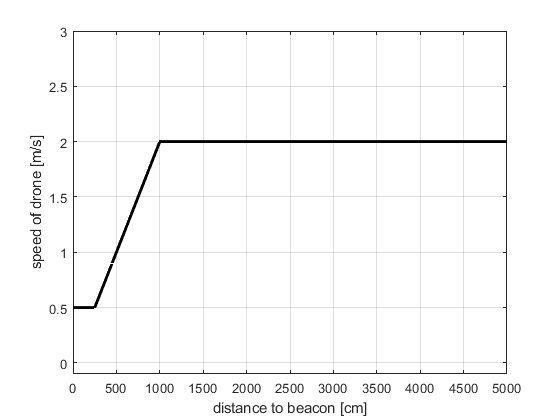
\includegraphics[width=1\columnwidth]{plot.png}}
\caption{speed of drone during beacon approach}
\label{fig-3}
\end{figure}


Since the beacons are potentially not at the surface of the avalanche, the vector follower needs to make sure that the drone stops before touching the snow. This is achieved by retrieving three corner points of the avalanche using rosparam and then calculating the plane equation coefficients (a,b,c,d) with them. By solving the resulting plane equation for z, we get the height of the avalanche for a given x and y position.
\begin{equation}
ax + by + cz + d = 0 \Rightarrow z = \frac{d-ax-by}{c}
\end{equation}

Using this it can easily be checked if the drone is keeping a minimum distance to the avalanche by verifying following equation.

\begin{equation}
{z}_{drone} - {z}_{plane} \geq {offset \_ to \_ plane} 
\end{equation}

If this equation is violated, the drone will continue to search for the beacon without being allowed to move further downwards.

\section{Visualization and approximation of Beacon Locations}
For visualizing the movement of the UAV, the environment and the approximated beacon locations within ROS the 3D visualization tool rviz is used. Therefore different marker messages are send to the rviz node on a multitude of locations within the code. The costume rviz display pictures the search area corners (green squares), transmitter positions and orientations (red squares), the UAV itself (blue UAV) as well as the drones trajectory (fine green line). The trajectory display is calculated by a external package. \cite{b4} If the UAV detects a beacon in sensor range, a red vector arrow based on the UAV marker indicates the flux vectors orientation.
During the execution of a mission markers (transparent blue spheres) are placed within the rviz environment whenever a transmitter is found as explained in section \ref{beacon simulation}. The position of a particular transmitter is calculated via the addition of the flux vector multiplied by the distance between receiver and transmitter to the current position of the receiver.

\begin{equation}
\bar{p}_{t, appr.}=\bar{p}_{r}+\bar{q}_{flux}\cdot d
\end{equation}

This fairly simple approximation results in quiet good results for appropriately small distance values due to the shape of the flux lines pointing to the transmitter in close proximity to the beacon. A location report containing the real beacon locations as well as all beacon locations calculated by the algorithm is printed to the terminal when the UAV returns to the starting point. A small survey with a sample size of 10 runs was conducted. Within the experiment four beacons where distributed over a searching area with fixed dimensions. The algorithm was able to find all 40 beacons. A averaged L1 error of 0.653 could be reached.

\section{Conclusion and Outlook}
Overall it could be shown that a simple pre-planned searching path, combined with the detection and following of the beacons flux lines is sufficient enough to find the "avalanche victims". The current approach only works on a mostly level area, but with additional sensors to measure the height above ground, more complex terrain could be covered. For victims that are buried deeper in the snow, more testing and development needs to be done.

As an outlook to further improvements we would like to reduce the time it takes to execute the pre-planned searching path. Due to the high number of waypoints and the mathematically intense nature of the minimum snap trajectory calculation, it takes a lot of time for the drone to start flying. We propose reducing the number of initial waypoints as well as calculating the trajectory continuously on the fly as opposed to once at the start.



\begin{thebibliography}{00}
\bibitem{b1} https://github.com/ethz-asl/mav\_trajectory\_generation
\bibitem{b2} P. Pinies and J. D. Tardos, "Fast localization of avalanche victims using sum of Gaussians," Proceedings 2006 IEEE International Conference on Robotics and Automation, 2006. ICRA 2006., 2006, pp. 3989-3994, doi: 10.1109/ROBOT.2006.1642314.

\bibitem{b3} J. Cacace, N. Mimmo and L. Marconi, "A ROS Gazebo plugin to simulate ARVA sensors," 2020 IEEE International Conference on Robotics and Automation (ICRA), 2020, pp. 7233-7239, doi: 10.1109/ICRA40945.2020.9196914.
\bibitem{b4} https://github.com/tu-darmstadt-ros-pkg/hector\_slam

\end{thebibliography}

\end{document}
